\documentclass[11pt]{article}
\usepackage{amsmath,amsfonts,amssymb,amsthm,fullpage}
\usepackage{graphicx}
\usepackage{float}
\usepackage{booktabs}
\usepackage{array}
\usepackage{enumitem}
\usepackage{pdflscape}
\usepackage{xcolor}
\usepackage{url}
\usepackage[hidelinks]{hyperref}
\usepackage{microtype}
\usepackage{caption}
\newcolumntype{L}[1]{>{\raggedright\arraybackslash}p{#1}}
\newcolumntype{C}[1]{>{\centering\arraybackslash}p{#1}}

\title{ISYE 6740 Summer 2026\\Final Project Report\\Detecting Overpriced Airbnb Listings Using Residual Modeling, Clustering, and Density Estimation}
\author{Sayeed Ahmed\\Project Group 059}
\date{}

\begin{document}
\maketitle

\section*{1. Introduction and Problem Statement}

Airbnb prices are easy to observe, but deciding whether a listing is fairly priced is not the same as simply sorting by the nightly rate. A large entire home in a central Austin neighborhood may reasonably charge much more than a small private room or a suburban unit. At the same time, two listings with similar location, size, room type, amenities, and review history can still have very different listed prices. This project studies that second case: listings that appear unusually expensive after adjusting for observable differences.

The goal of the project is not to prove that a host is intentionally overcharging. Instead, I treat overpricing as a screening problem. I first estimate a fair expected nightly price from the available listing information. I then study the residual
\[
 r_i = \log(p_i)-\widehat{\log(p_i)},
\]
where $p_i$ is the actual listed nightly price for listing $i$. A large positive residual means that the listing is priced above what the model expects. The final ranking gives more weight to listings that also look unusual within peer groups and show weaker demand-proxy signals, such as high future availability or low recent review activity.

This setup made sense for this project because it combines supervised and unsupervised learning. The supervised part estimates expected price. The unsupervised part uses PCA, K-means clustering, and Gaussian mixture density scoring to compare listings to similar listings rather than judging the entire Austin market under one standard. This follows the original proposal idea, where prediction was only the first layer and the more interesting part was residual and peer-group analysis.

The main contribution is the way these pieces are put together. This is not only a price-prediction project. The prediction model is used to define a fair-price residual, then that residual is compared within peer groups and combined with density and demand-proxy signals. That gives a more practical ranking than simply sorting by price or by model error alone.

\paragraph{Team contribution.} This was a solo project. I was responsible for collecting the data, cleaning it, building the features, training the models, creating the residual and clustering scores, checking the results, and preparing the final report.

\section*{2. Data Source and Preprocessing}

The data came from Inside Airbnb for Austin, Texas \cite{insideairbnb_data}. The project used the public listing, calendar, and review files. The detailed listing file was the main source for price and property features. Calendar data was aggregated to listing-level availability and stay-rule features. Review data was aggregated into activity features such as total review count, recent review count, and days since last review. I also kept the usual caveat from the Inside Airbnb assumptions: reviews and calendar availability are useful proxies, but they are not the same as true booking records \cite{insideairbnb_assumptions}.

The initial cleaning step removed duplicate listing IDs, listings with missing or nonpositive prices, listings above the 99.5th percentile of price, invalid coordinates, and implausible capacity, bedroom, bed, and bathroom values. The final cleaned listing table had 10,230 listings. The calendar file had 11,320 listing IDs, and every cleaned listing had a calendar match. The review file had 9,451 listing IDs, with 8,616 matching the cleaned listing table. Listings without review history were kept and given review-count features equal to zero.

One practical data issue was that the Austin calendar file did not contain calendar-level price columns such as \texttt{price} or \texttt{adjusted\_price}. Because of that, I used calendar data for availability and minimum/maximum night rules, not for seasonal price variation. This was a change from the initial plan, but it does not affect the main residual modeling idea because the actual nightly price still comes from the detailed listing file.

\begin{table}[H]
\centering
\caption{Main data tables after cleaning and aggregation.}
\small
\begin{tabular}{L{0.20\textwidth}rL{0.18\textwidth}L{0.42\textwidth}}
\toprule
Dataset & Rows & Main role & Notes \\
\midrule
Cleaned listings & 10,230 & Modeling table & Price, location, property, host, review-score, and amenity fields \\
Calendar features & 11,320 & Availability proxy & All cleaned listings had calendar matches \\
Review features & 9,451 & Activity proxy & 8,616 cleaned listings had review matches \\
Final modeling table & 10,230 & Model input & One row per cleaned listing \\
\bottomrule
\end{tabular}
\end{table}

Prices were modeled on the log scale because nightly prices were strongly right-skewed. Amenity text was parsed into indicator variables for common features such as Wi-Fi, kitchen, parking, pool, hot tub, washer/dryer, air conditioning, and dedicated workspace. Categorical fields such as room type, property type, neighborhood, and capacity bucket were used as model inputs through one-hot encoding. Numeric fields were imputed and standardized where needed.

The implementation was organized as a reproducible script pipeline instead of one manual notebook. Separate scripts cleaned the listings, built calendar features, built review features, merged the modeling table, generated EDA tables and figures, trained the fair-price models, scored residuals, ran PCA/clustering/density scoring, created the final ranked candidates, and produced validation summaries. This also made it easier to rerun the project after discovering that the calendar file did not contain price columns.

\section*{3. Exploratory Data Analysis}

The final modeling table had a median nightly price of \$216 and a mean nightly price of \$311.58. This gap already shows that the price distribution is right-skewed, with a smaller number of expensive listings pulling the mean upward. Entire-home listings dominated the Austin data, with 8,464 of the 10,230 cleaned listings. Private rooms were the second largest group, while hotel rooms and shared rooms were much smaller groups.

\begin{table}[H]
\centering
\caption{Price and activity summary by room type.}
\small
\begin{tabular}{lrrrr}
\toprule
Room type & Listings & Median price & Mean price & Median reviews (365d) \\
\midrule
Entire home/apt & 8,464 & \$231.50 & \$333.32 & 7.0 \\
Private room & 1,511 & \$95.33 & \$166.68 & 1.0 \\
Hotel room & 184 & \$310.50 & \$611.99 & 0.0 \\
Shared room & 71 & \$16.81 & \$25.20 & 1.0 \\
\bottomrule
\end{tabular}
\end{table}

The strongest simple correlations with log price were capacity-related variables. The correlation with \texttt{accommodates} was 0.644, followed by bedrooms, bathrooms, and beds. This is intuitive because larger listings can usually charge more. Minimum nights had a negative correlation with log price, which suggests that long-stay or monthly-style listings behave differently from ordinary nightly rentals. Amenity count also had a positive relationship with price.

\begin{figure}[H]
\centering
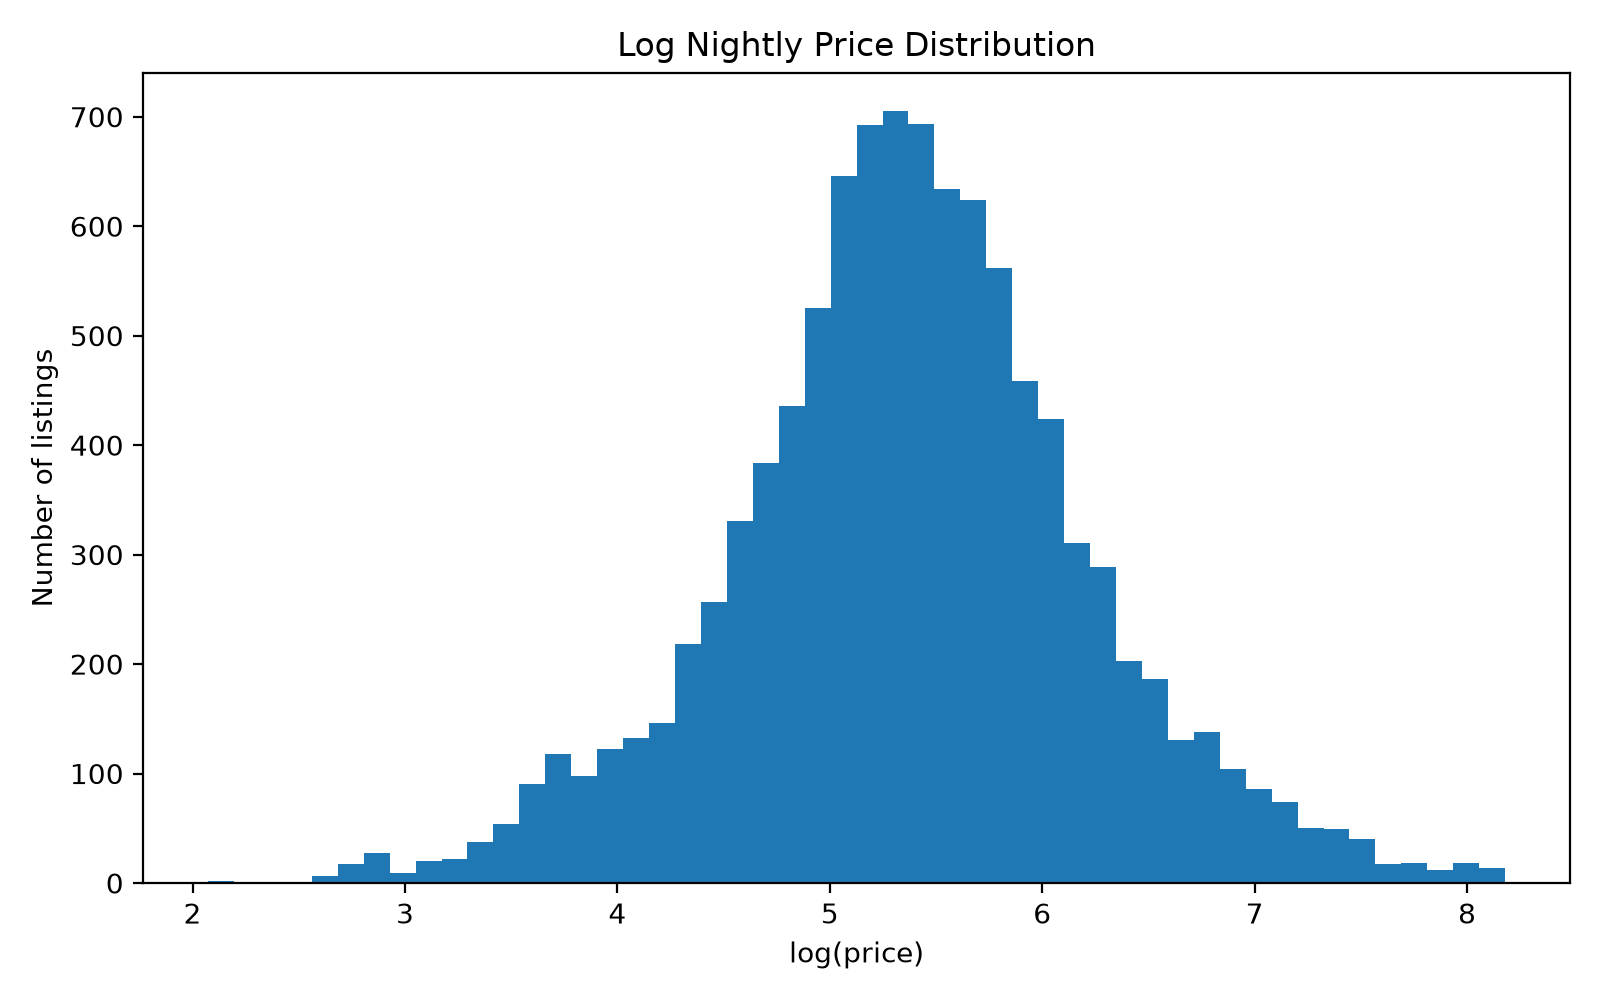
\includegraphics[width=0.78\textwidth]{figures/eda/log_price_distribution.png}
\caption{Distribution of log nightly price after cleaning.}
\label{fig:log_price_distribution}
\end{figure}

\begin{figure}[H]
\centering
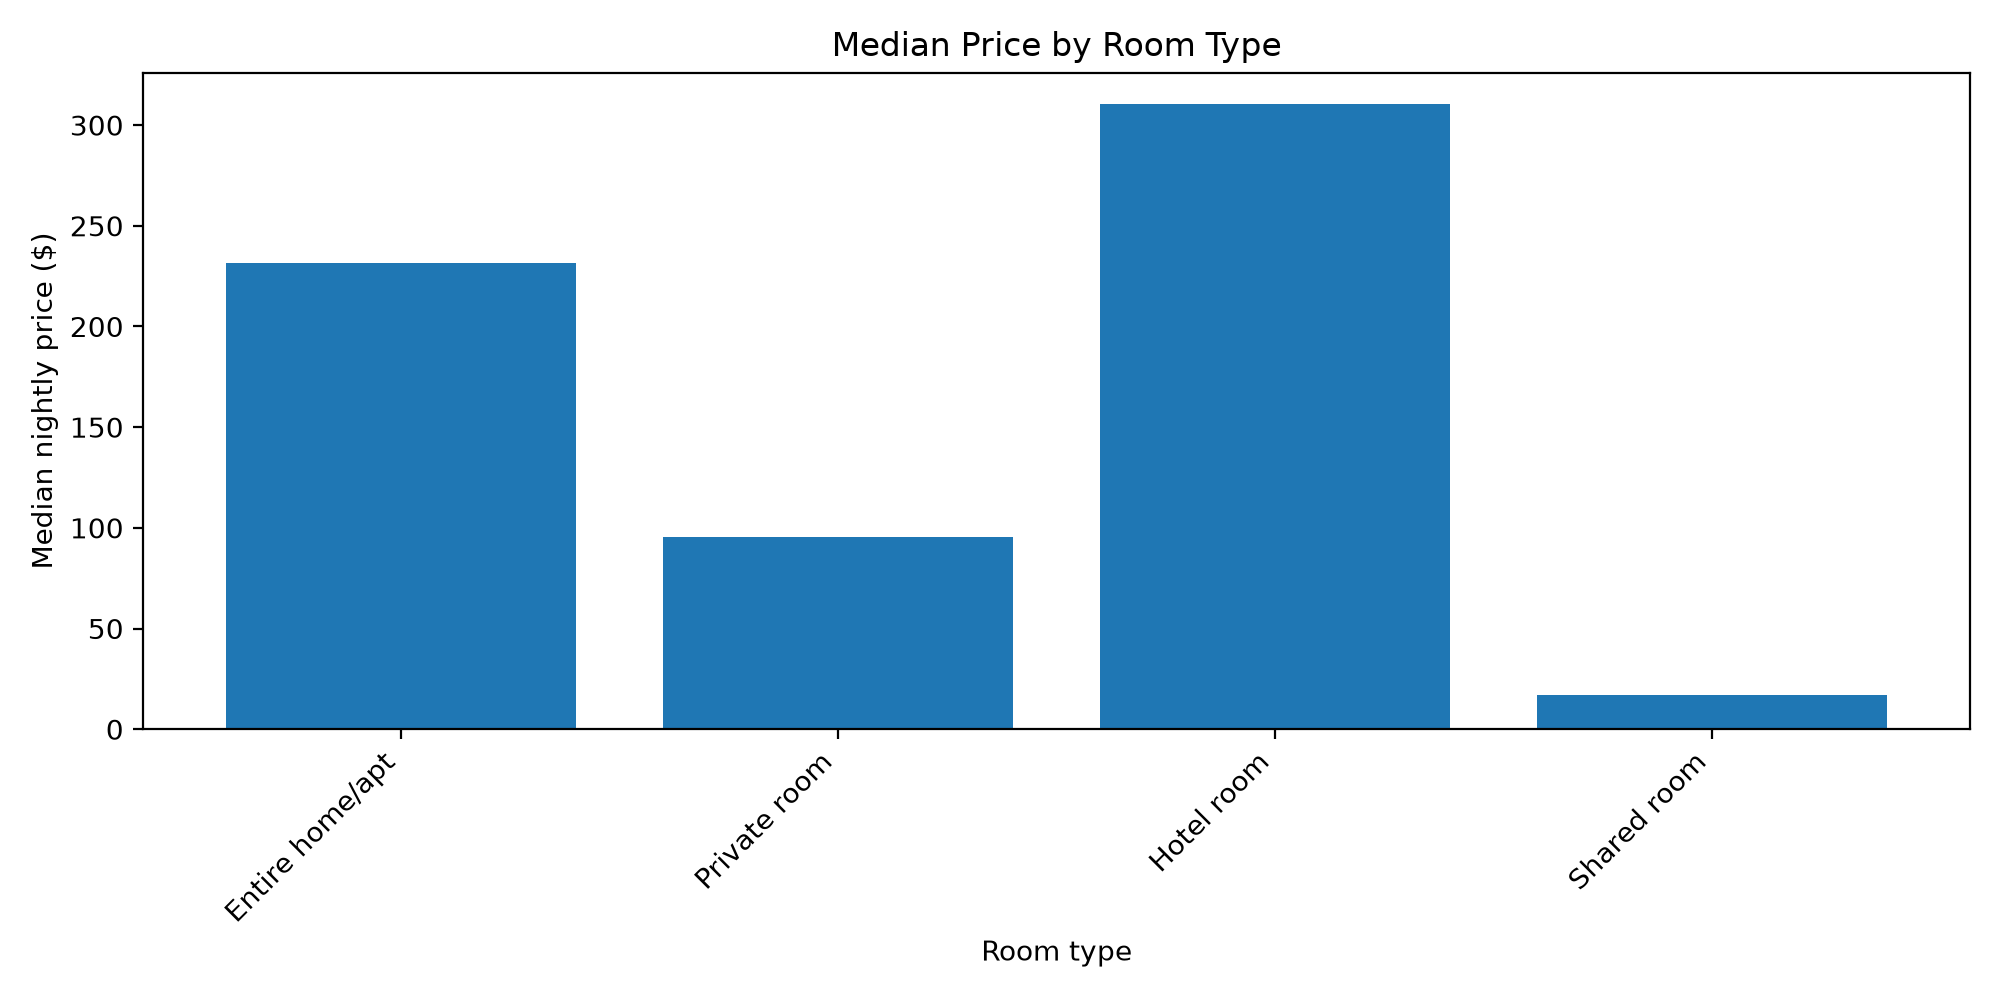
\includegraphics[width=0.78\textwidth]{figures/eda/median_price_by_room_type.png}
\caption{Median price by room type. Entire homes and hotel rooms have much higher prices than private or shared rooms.}
\label{fig:price_room_type}
\end{figure}

\section*{4. Fair-Price Modeling}

The first modeling step was to estimate expected nightly price. I compared simple median baselines with linear regression, Ridge regression, Lasso regression, random forest, and gradient boosting. Random forest and gradient boosting were included as practical nonlinear models, using the original methods as references \cite{breiman_randomforest,friedman_boosting}. The target variable was $\log(\text{price})$. The general supervised-learning framing follows standard statistical learning practice \cite{esl}. The simple baselines were included because a useful model should clearly beat basic rules such as neighborhood-room-type median price.

Using $y_i=\log(p_i)$ and feature vector $x_i$, the fair-price model can be written as estimating a function $f_\theta(x_i)$ that predicts expected log price. In general form, the training problem was
\[
    \min_{\theta} \frac{1}{n} \sum_{i=1}^{n} \left(y_i - f_\theta(x_i)\right)^2.
\]
For the linear and regularized models, this reduces to estimating coefficients for the feature vector. For the tree-based models, the same prediction goal is used, but the fitted function is nonlinear.

Gradient boosting was the best trained model on the held-out test set. It had test RMSE of 0.3190 on the log-price scale and MAE of \$79.63 on the dollar scale. The best simple baseline was the neighborhood plus room type plus capacity median, with RMSE of 0.5547 and MAE of \$126.83. Relative to that best baseline, gradient boosting improved log-RMSE by 42.48\% and dollar MAE by 37.21\%. This is strong enough to use the model residuals as the starting point for overpricing analysis.

\begin{table}[H]
\centering
\caption{Model comparison on the held-out test set.}
\small
\begin{tabular}{L{0.43\textwidth}rrrr}
\toprule
Model & RMSE log & MAE price & $R^2$ log & MAPE \\
\midrule
Gradient boosting & 0.3190 & \$79.63 & 0.8526 & 23.26\% \\
Random forest & 0.3649 & \$91.81 & 0.8071 & 27.10\% \\
Lasso regression & 0.3835 & \$96.88 & 0.7869 & 29.18\% \\
Ridge regression & 0.3836 & \$96.61 & 0.7868 & 29.27\% \\
Linear regression & 0.3852 & \$96.83 & 0.7851 & 29.44\% \\
Neighborhood + room type + capacity median & 0.5547 & \$126.83 & 0.5543 & 43.92\% \\
Overall median & 0.8313 & \$181.43 & -0.0010 & 81.88\% \\
\bottomrule
\end{tabular}
\end{table}

The most important predictors also made sense. The top permutation-importance variables included accommodates, minimum-night rules, bathrooms, room type, latitude, longitude, bedrooms, property type, neighborhood, days since last review, pool indicator, and amenity count. This helps support the model because the largest drivers are variables that should reasonably matter in Airbnb pricing.

\begin{figure}[H]
\centering
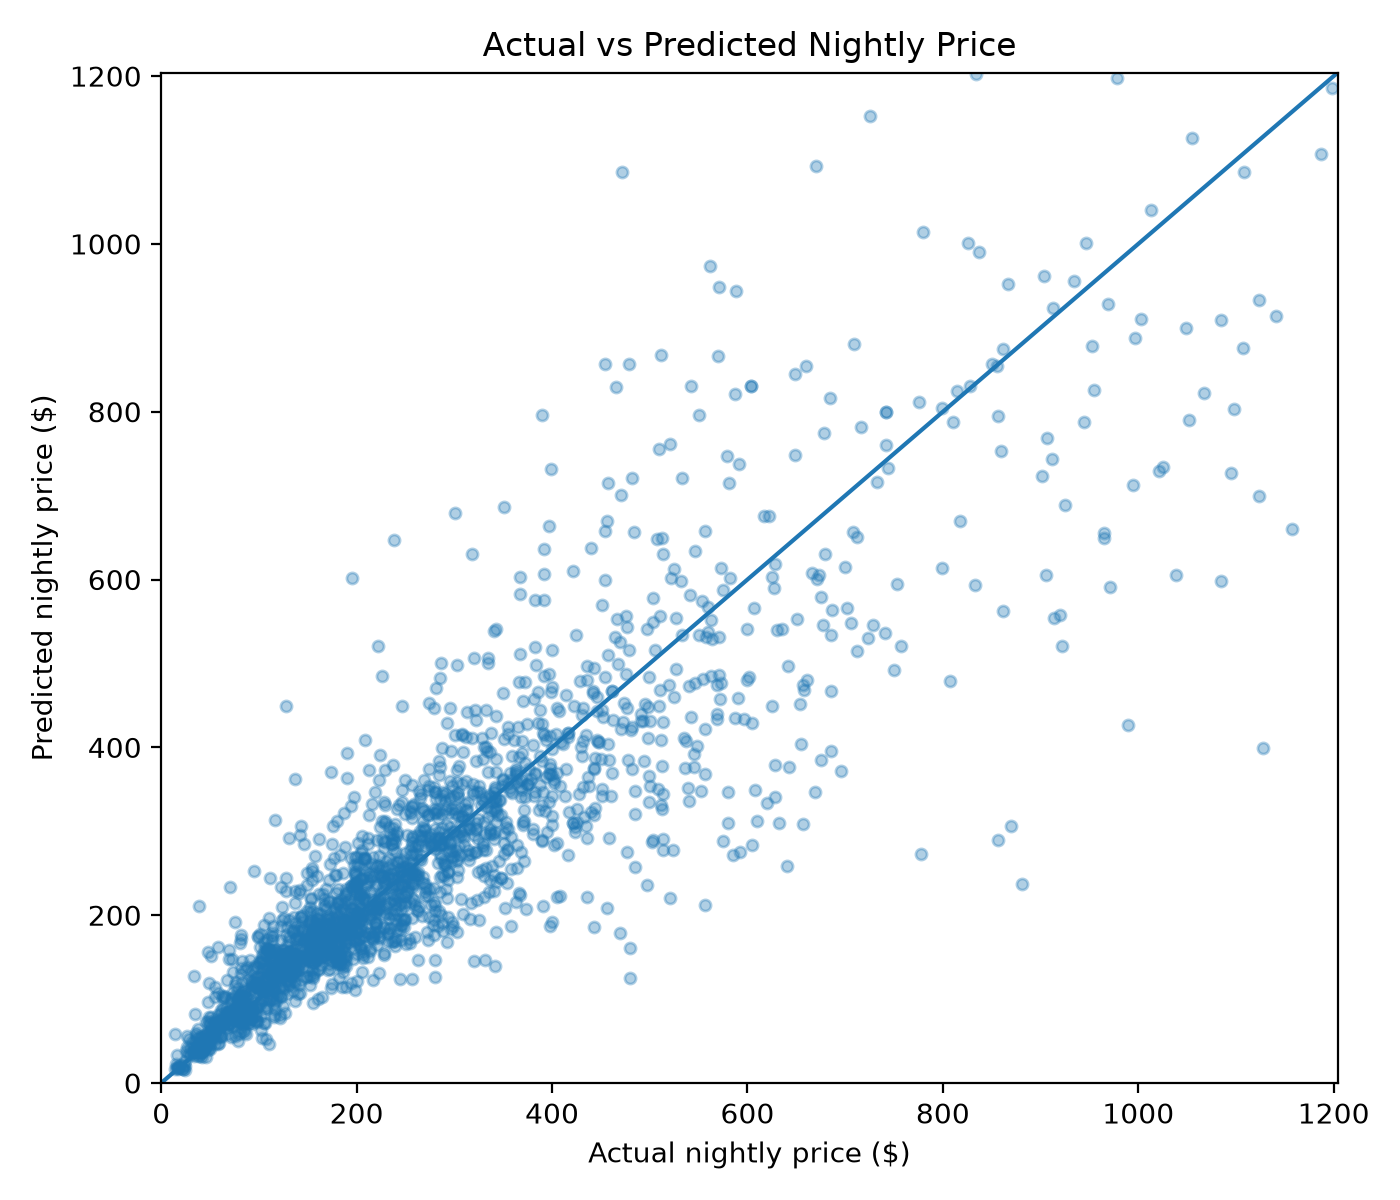
\includegraphics[width=0.76\textwidth]{figures/model_eval/actual_vs_predicted_price.png}
\caption{Actual versus predicted nightly prices for the selected fair-price model.}
\label{fig:actual_predicted}
\end{figure}

\begin{figure}[H]
\centering
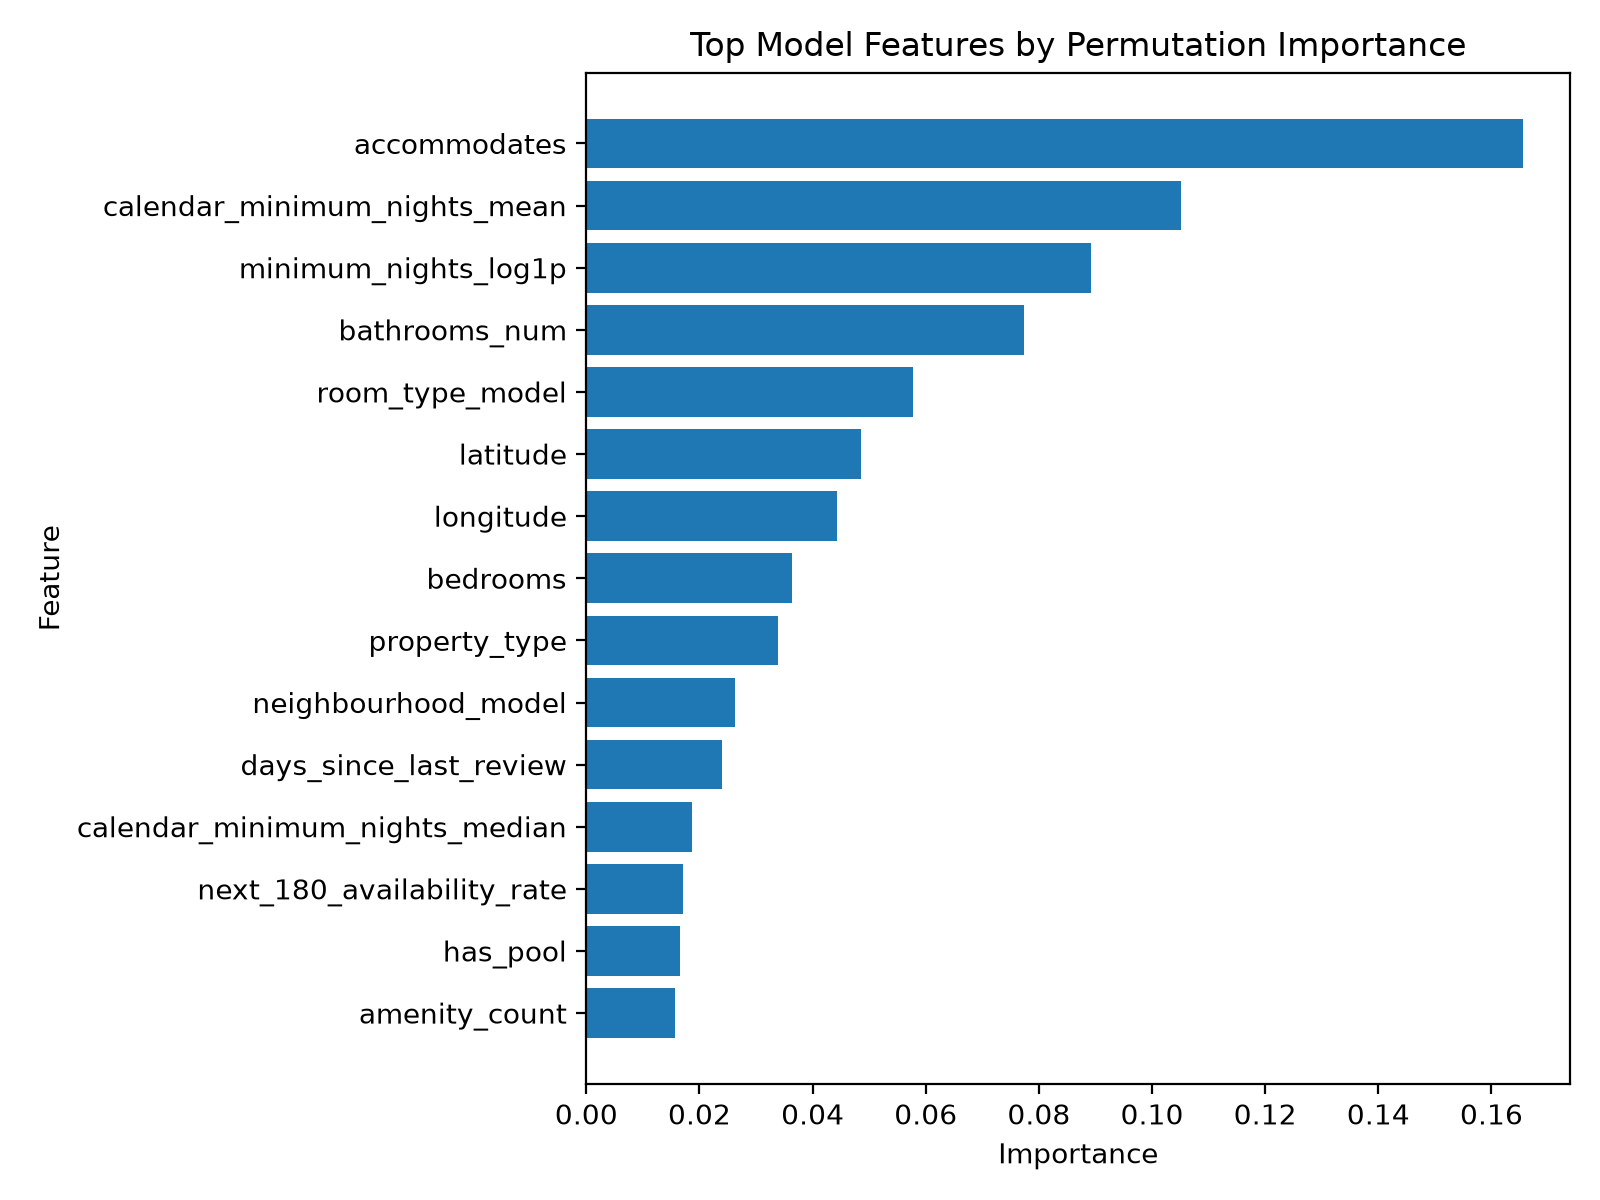
\includegraphics[width=0.76\textwidth]{figures/model_eval/top_feature_importance.png}
\caption{Top features by permutation importance for the selected model.}
\label{fig:feature_importance}
\end{figure}

\section*{5. Residual and Peer-Group Overpricing Score}

After selecting the fair-price model, I generated out-of-fold predictions for every listing. I used out-of-fold residuals so that each listing's residual was based on a model that did not train on that listing. This makes the residual score less optimistic than scoring every listing with a model fit on the full data.

The raw residual was
\[
 r_i = \log(p_i)-\widehat{\log(p_i)}.
\]
A positive value means the listing is above expected price. To avoid simply flagging expensive listings, I also standardized residuals within two peer-group definitions. The first peer group used neighborhood and room type. The second used neighborhood, room type, and capacity bucket. The residual signal score was a weighted average of three percentile ranks:
\[
S^{\text{resid}}_i
=0.40S^{\text{global}}_i
+0.30S^{\text{simple peer}}_i
+0.30S^{\text{capacity peer}}_i.
\]
This keeps the score interpretable while still comparing a listing against both the full market and closer peers.

The peer scoring created 101 simple peer groups and 303 capacity peer groups. Small peer groups were handled using a global fallback score so that tiny segments would not produce unstable percentiles. The top residual candidates were often listings whose prices were several times larger than their predicted prices. Some looked like special cases, such as long-stay or unusual rental formats, which is a reminder that the ranking is a screening tool rather than a final judgment.

\begin{figure}[H]
\centering
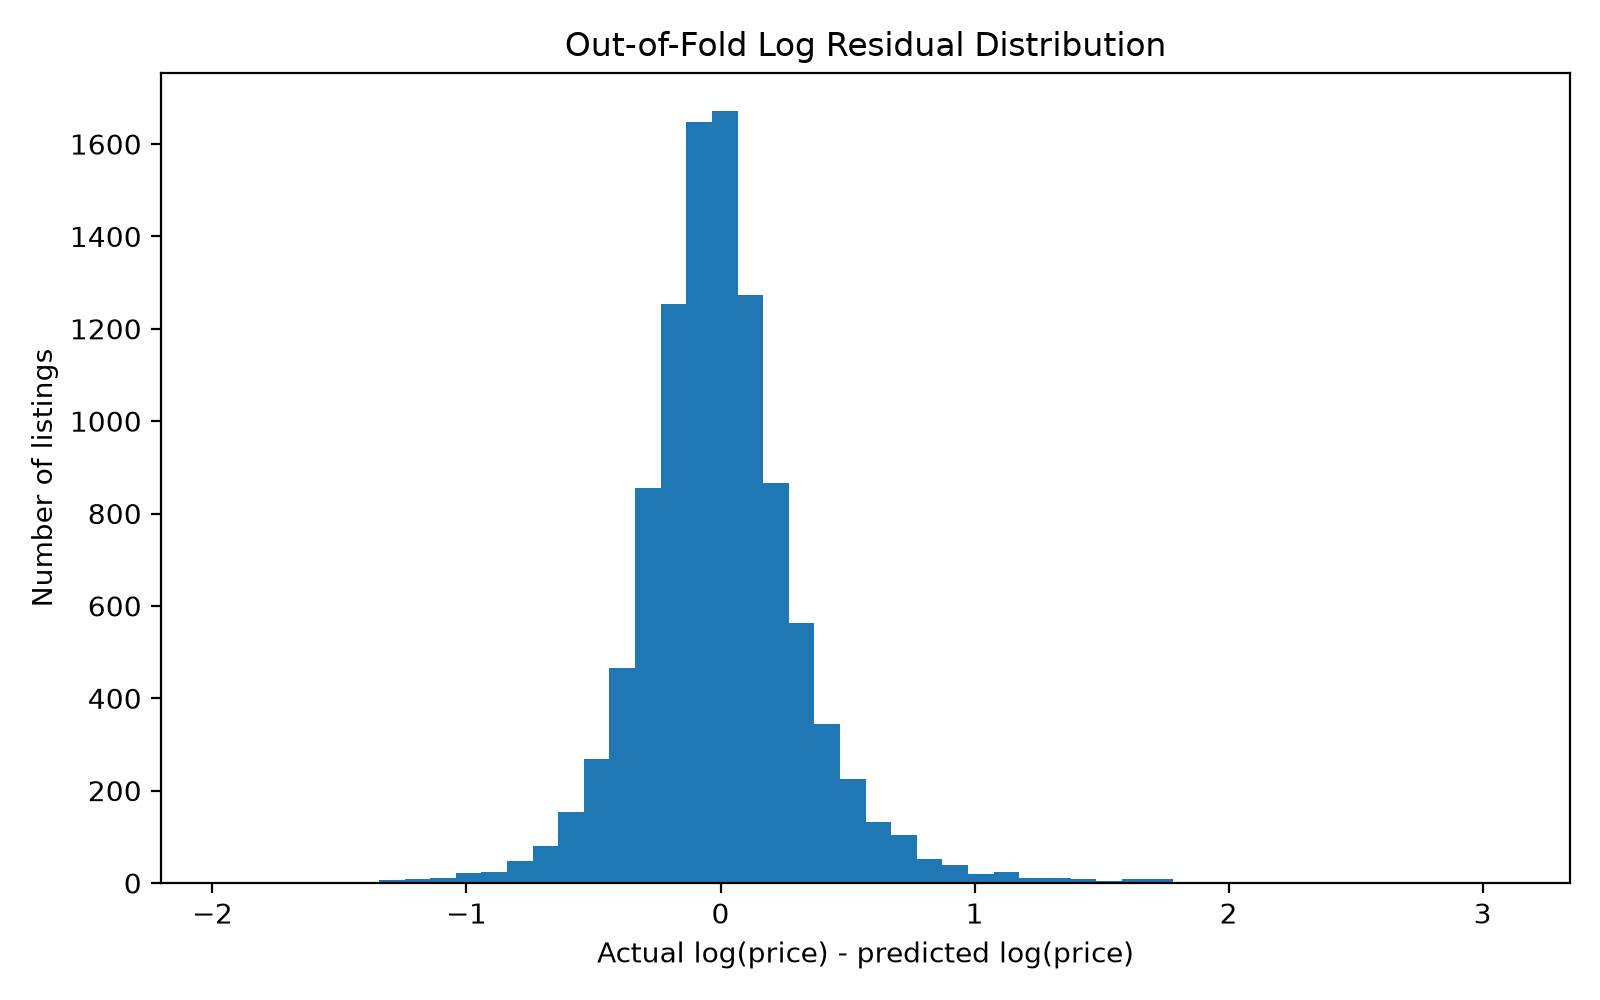
\includegraphics[width=0.76\textwidth]{figures/model_eval/oof_log_residual_distribution.png}
\caption{Out-of-fold log residual distribution from the selected fair-price model.}
\label{fig:residual_distribution}
\end{figure}

\section*{6. PCA, K-Means Clustering, and Density Scoring}

The next step used course-related unsupervised methods to compare listings in a feature space. Numeric variables were imputed and standardized, categorical variables were one-hot encoded, and PCA was used to project the listing features into a lower-dimensional representation. These PCA, K-means, density-estimation, GMM, and optimization steps were chosen to stay close to the course material \cite{course_notes}. I kept 15 principal components, which explained 75.21\% of the processed feature variance. This was enough to summarize much of the structure without using every encoded feature directly in clustering.

K-means was run in PCA space for several candidate values of $k$. In the notation from lecture, the clustering step tries to choose clusters and centroids that minimize within-cluster squared distance:
\[
    \min_{C_1,\ldots,C_k} \sum_{j=1}^{k} \sum_{z_i \in C_j} \left\| z_i - \mu_j \right\|^2,
\]
where $z_i$ is the PCA feature vector for listing $i$. The selected value was $k=7$, based on the largest silhouette score among the tested choices. The silhouette scores were not very high, so I interpret the clusters as useful peer segments rather than perfectly separated market groups. This is reasonable for Airbnb data because listings vary along many overlapping dimensions.

\begin{table}[H]
\centering
\caption{K-means model selection in PCA space.}
\begin{tabular}{rrr}
\toprule
$k$ & Inertia & Silhouette score \\
\midrule
4 & 290317.76 & 0.1511 \\
5 & 267071.02 & 0.1571 \\
6 & 244121.13 & 0.1552 \\
7 & 225558.65 & 0.1571 \\
8 & 215960.04 & 0.1519 \\
9 & 205601.26 & 0.1571 \\
10 & 199725.59 & 0.1560 \\
12 & 185264.13 & 0.1324 \\
\bottomrule
\end{tabular}
\end{table}

A density-based anomaly score was then created using a Gaussian mixture model in PCA space. This is related to the GMM and EM material from lecture. In this step, the density of a listing's PCA vector was modeled as
\[
    p(z_i)=\sum_{m=1}^{K} \pi_m \mathcal{N}(z_i \mid \mu_m, \Sigma_m),
\]
where each component represents one Gaussian-shaped part of the feature space. I did not use KDE in the final implementation. GMM was simpler to run on the full dataset and gave a direct log-density score for each listing. The implementation used scikit-learn for the modeling pipeline \cite{sklearn}. A listing with low estimated density received a high anomaly percentile. The final cluster anomaly score averaged the K-means distance percentile and the GMM anomaly percentile:
\[
S^{\text{cluster}}_i
=0.50S^{\text{kmeans distance}}_i
+0.50S^{\text{GMM anomaly}}_i.
\]

\begin{figure}[H]
\centering
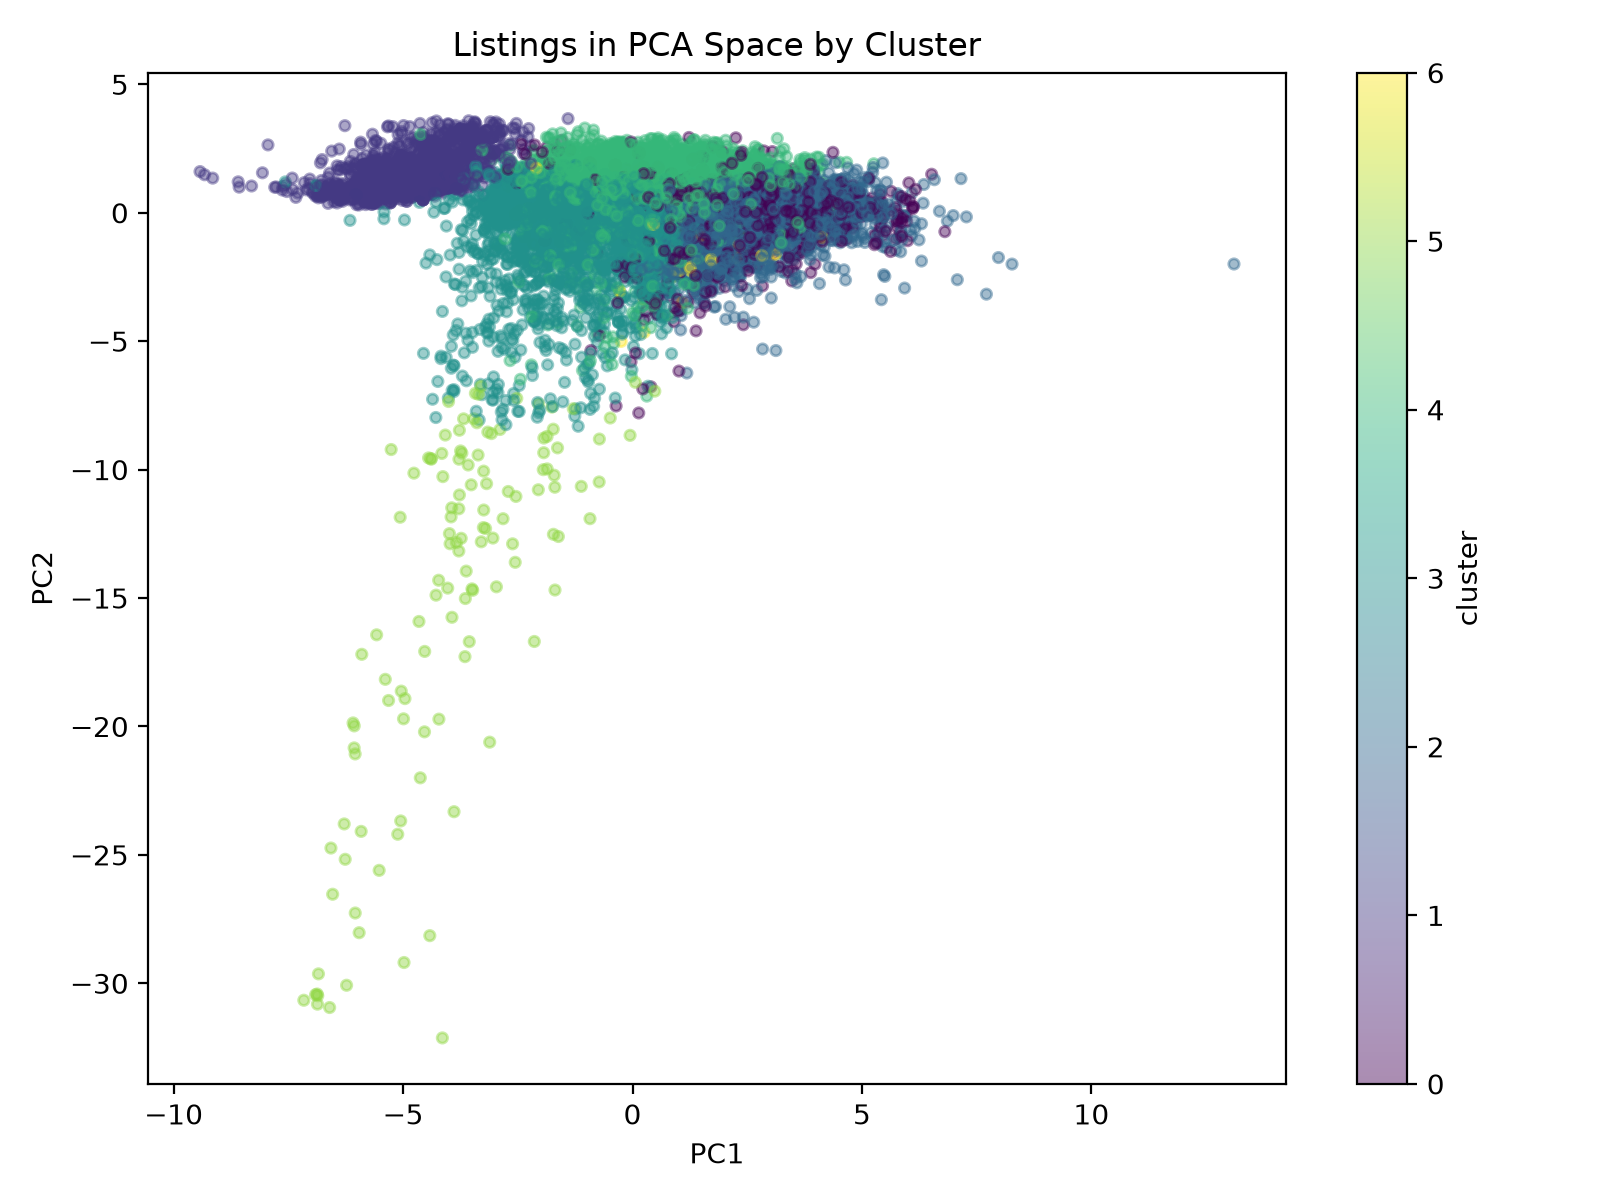
\includegraphics[width=0.78\textwidth]{figures/clustering/pca_cluster_scatter.png}
\caption{Listings plotted in the first two PCA directions and colored by K-means cluster.}
\label{fig:pca_cluster}
\end{figure}

\begin{figure}[H]
\centering
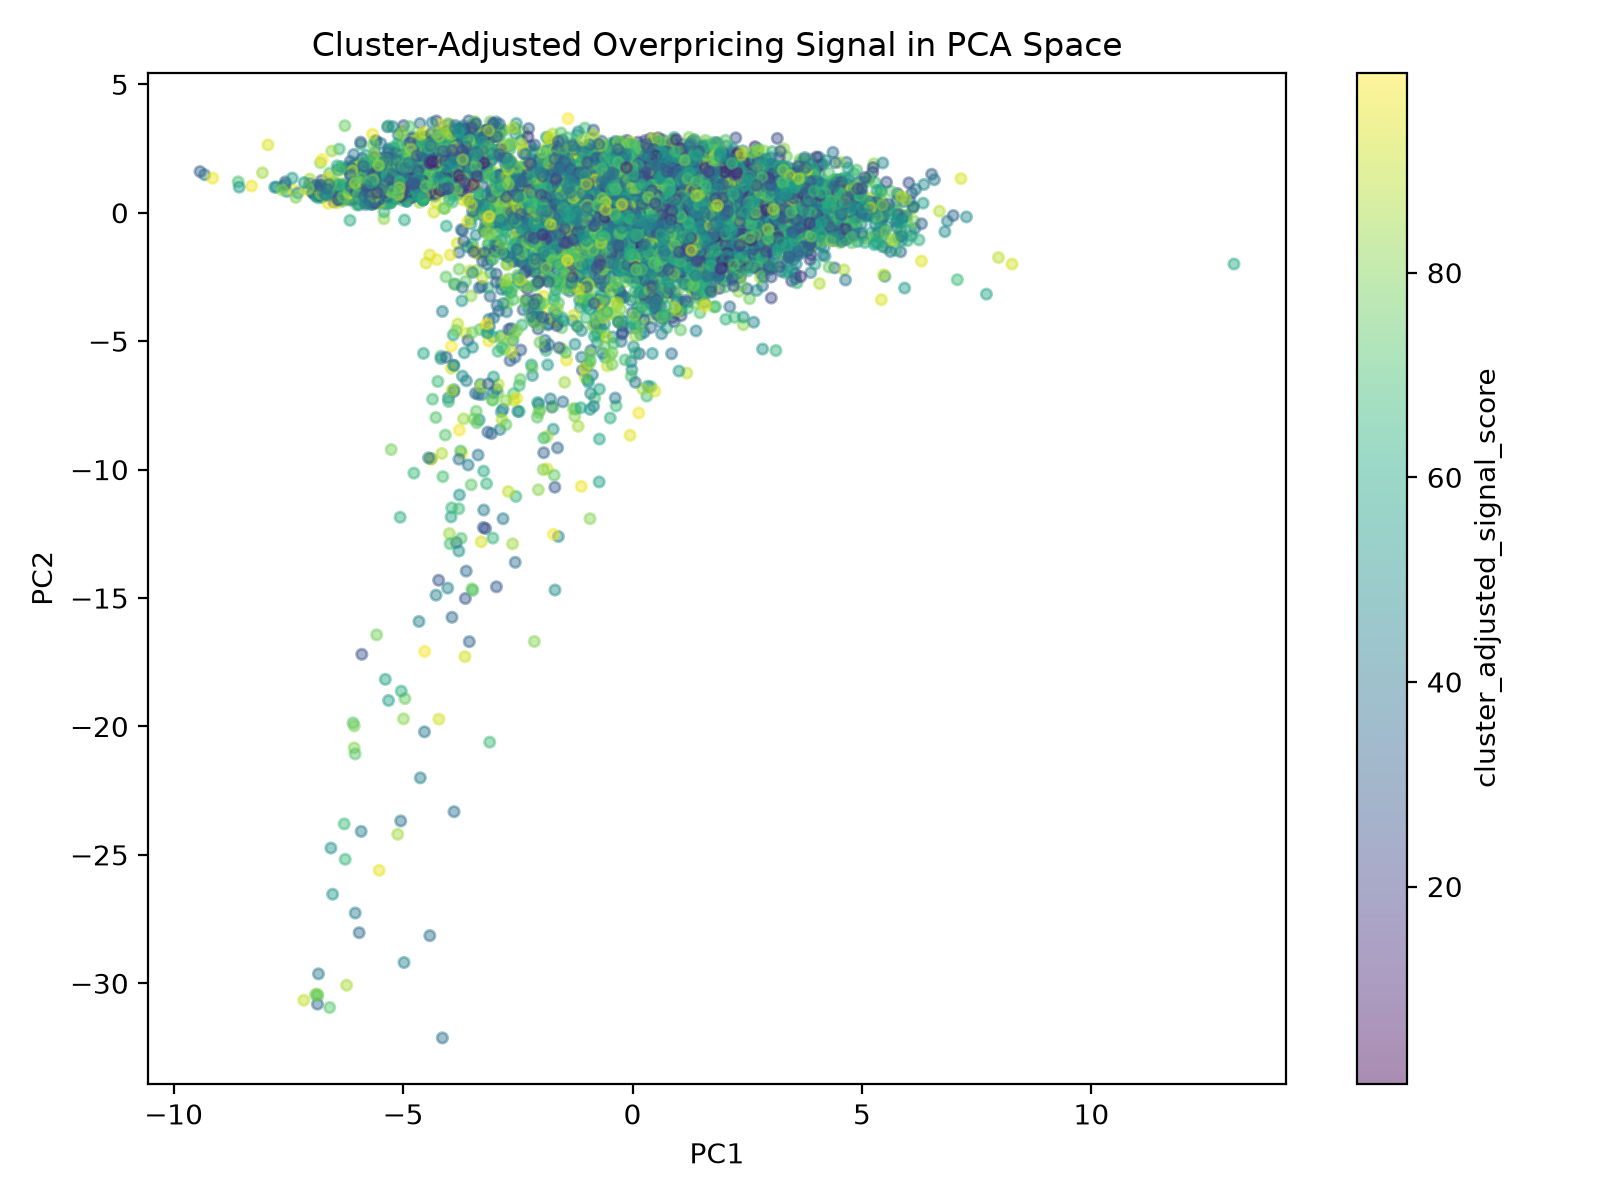
\includegraphics[width=0.78\textwidth]{figures/clustering/pca_cluster_adjusted_signal.png}
\caption{Cluster-adjusted overpricing signal in PCA space. Higher values mark listings that are both high-residual and unusual in feature space.}
\label{fig:pca_signal}
\end{figure}

\section*{7. Final Overpricing Ranking and Validation}

The final score combined the residual signal, cluster anomaly score, and demand-proxy score:
\[
S^{\text{final}}_i
=0.60S^{\text{resid}}_i
+0.25S^{\text{cluster}}_i
+0.15S^{\text{demand}}_i.
\]
The demand-proxy score used future availability and low recent review activity. Specifically, high availability increased the score, and listings with fewer recent reviews also received a higher demand-proxy score. These signals do not prove weak demand, but they are useful as supporting evidence because there is no official overpricing label in the data.

The final scoring produced 13 strong candidates, 62 moderate candidates, 533 watchlist listings, and 9,622 listings that were not flagged. Strong candidates had a median actual price of \$563.67 and a median predicted price of \$217.22. They were also highly available, with median availability of 1.00, and had median recent reviews equal to zero. This is the most important practical result of the project: the strongest candidates were not just expensive, but expensive relative to model expectation and weak on demand-side proxies.

\begin{table}[H]
\centering
\caption{Summary by final candidate label.}
\small
\begin{tabular}{L{0.24\textwidth}rrrrr}
\toprule
Candidate label & Listings & Actual & Predicted & \% above & Avail. \\
\midrule
Strong candidate & 13 & \$563.67 & \$217.22 & 124.54\% & 1.0000 \\
Moderate candidate & 62 & \$554.00 & \$230.78 & 111.12\% & 0.9836 \\
Watchlist & 533 & \$379.50 & \$222.52 & 60.61\% & 0.8685 \\
Not flagged & 9,622 & \$210.00 & \$217.50 & -3.52\% & 0.7260 \\
\bottomrule
\end{tabular}
\end{table}

The final score deciles also show the expected pattern. The top final-score decile had median actual price \$356.50, median predicted price \$220.88, and median percent above expected of 53.71\%. It also had median availability rate 0.8685 and median reviews in the last 365 days equal to 1. Lower deciles had much lower or negative percent-above-expected values.

\begin{table}[H]
\centering
\caption{Selected final-score decile results.}
\small
\begin{tabular}{rrrrr}
\toprule
Decile & Actual & Predicted & \% above & Recent reviews \\
\midrule
1 & \$181.00 & \$258.00 & -29.96\% & 13.0 \\
3 & \$169.00 & \$200.48 & -15.88\% & 7.0 \\
5 & \$203.76 & \$214.81 & -4.30\% & 6.0 \\
7 & \$229.00 & \$208.22 & 8.57\% & 6.0 \\
9 & \$293.00 & \$215.89 & 28.94\% & 3.0 \\
10 & \$356.50 & \$220.88 & 53.71\% & 1.0 \\
\bottomrule
\end{tabular}
\end{table}

\begin{figure}[H]
\centering
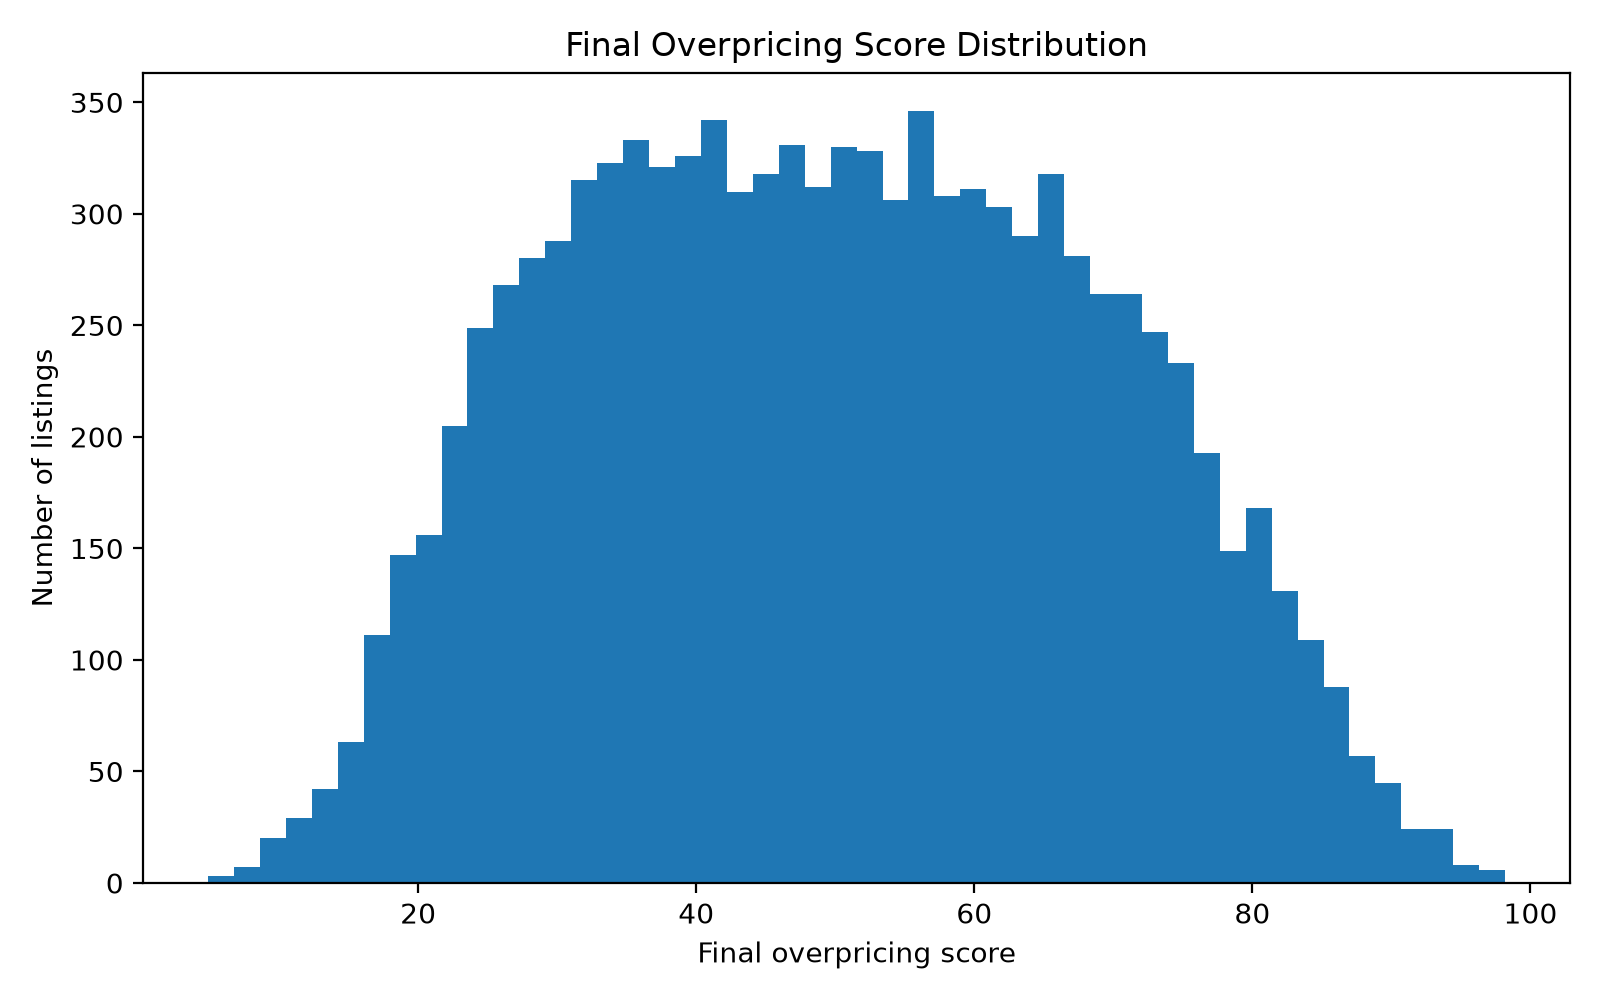
\includegraphics[width=0.76\textwidth]{figures/final/final_overpricing_score_distribution.png}
\caption{Distribution of the final overpricing score.}
\label{fig:final_score_distribution}
\end{figure}

\begin{figure}[H]
\centering
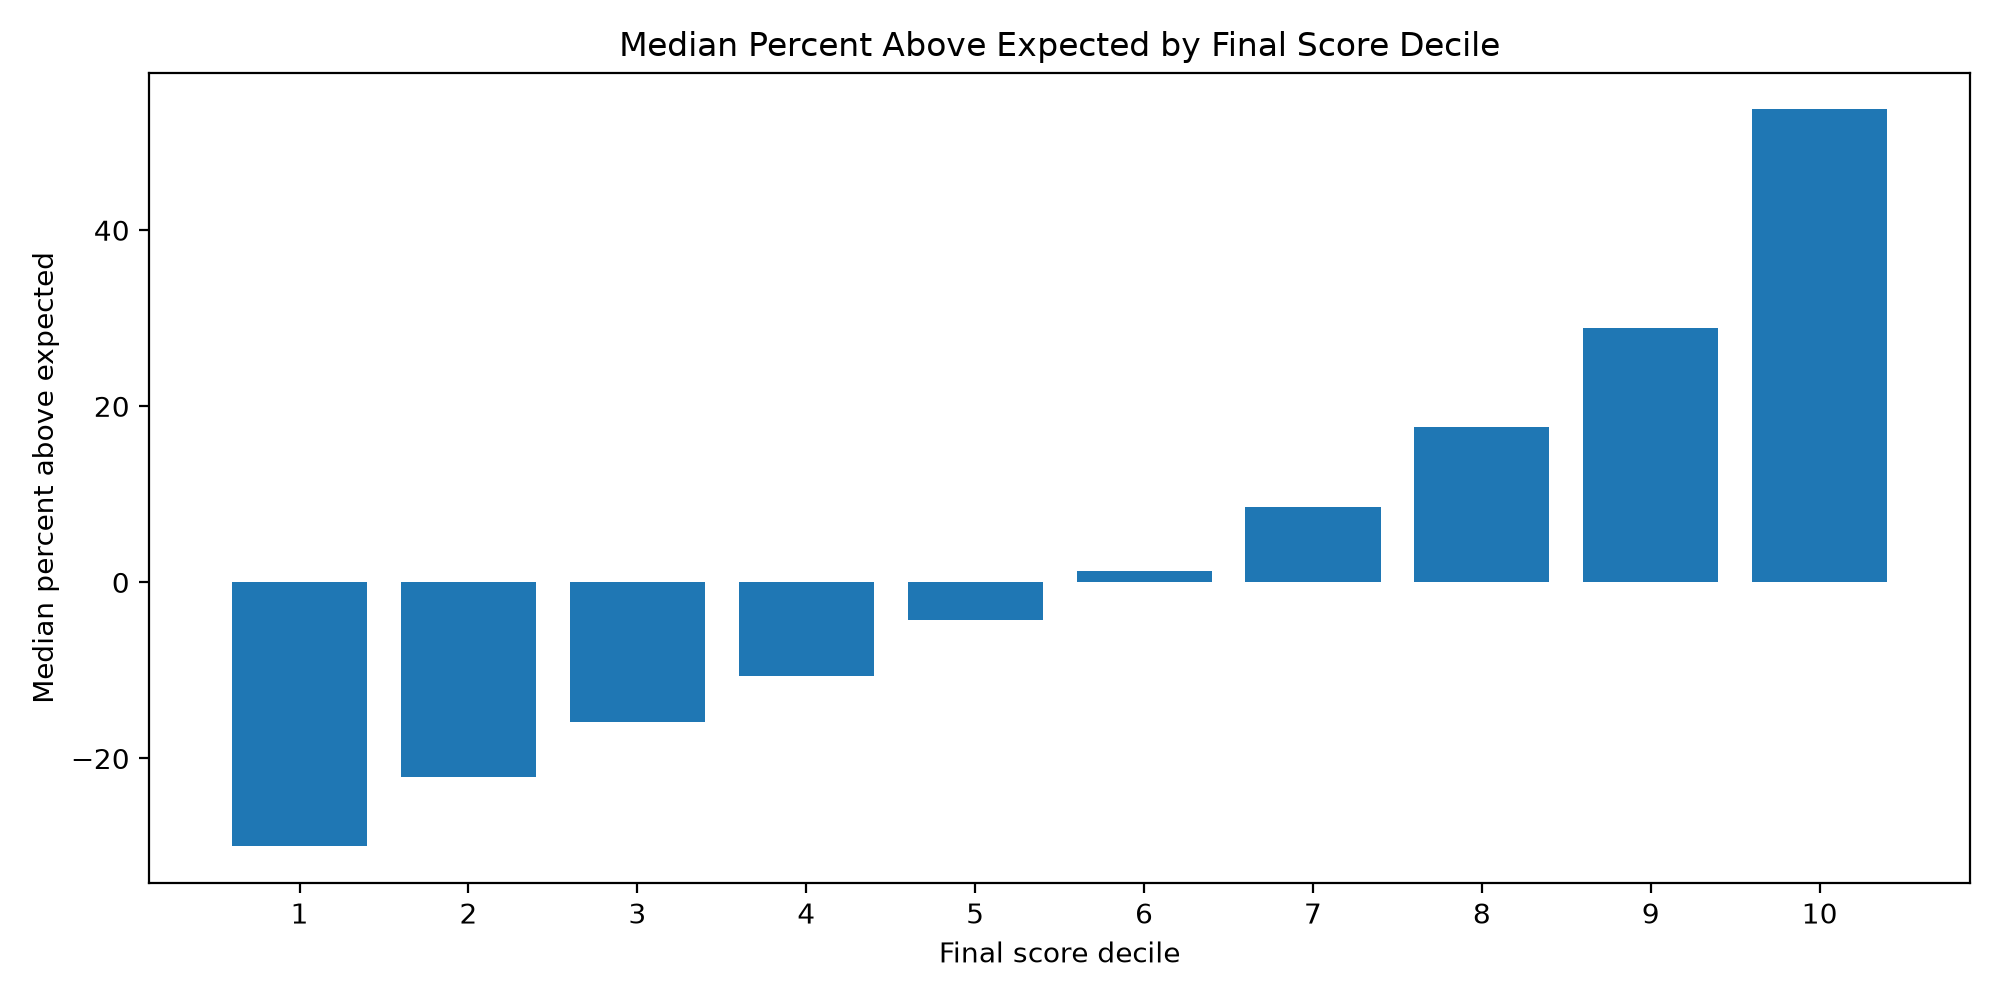
\includegraphics[width=0.76\textwidth]{figures/final/decile_vs_percent_above_expected.png}
\caption{Median percent above expected price by final-score decile.}
\label{fig:decile_percent}
\end{figure}

\begin{figure}[H]
\centering
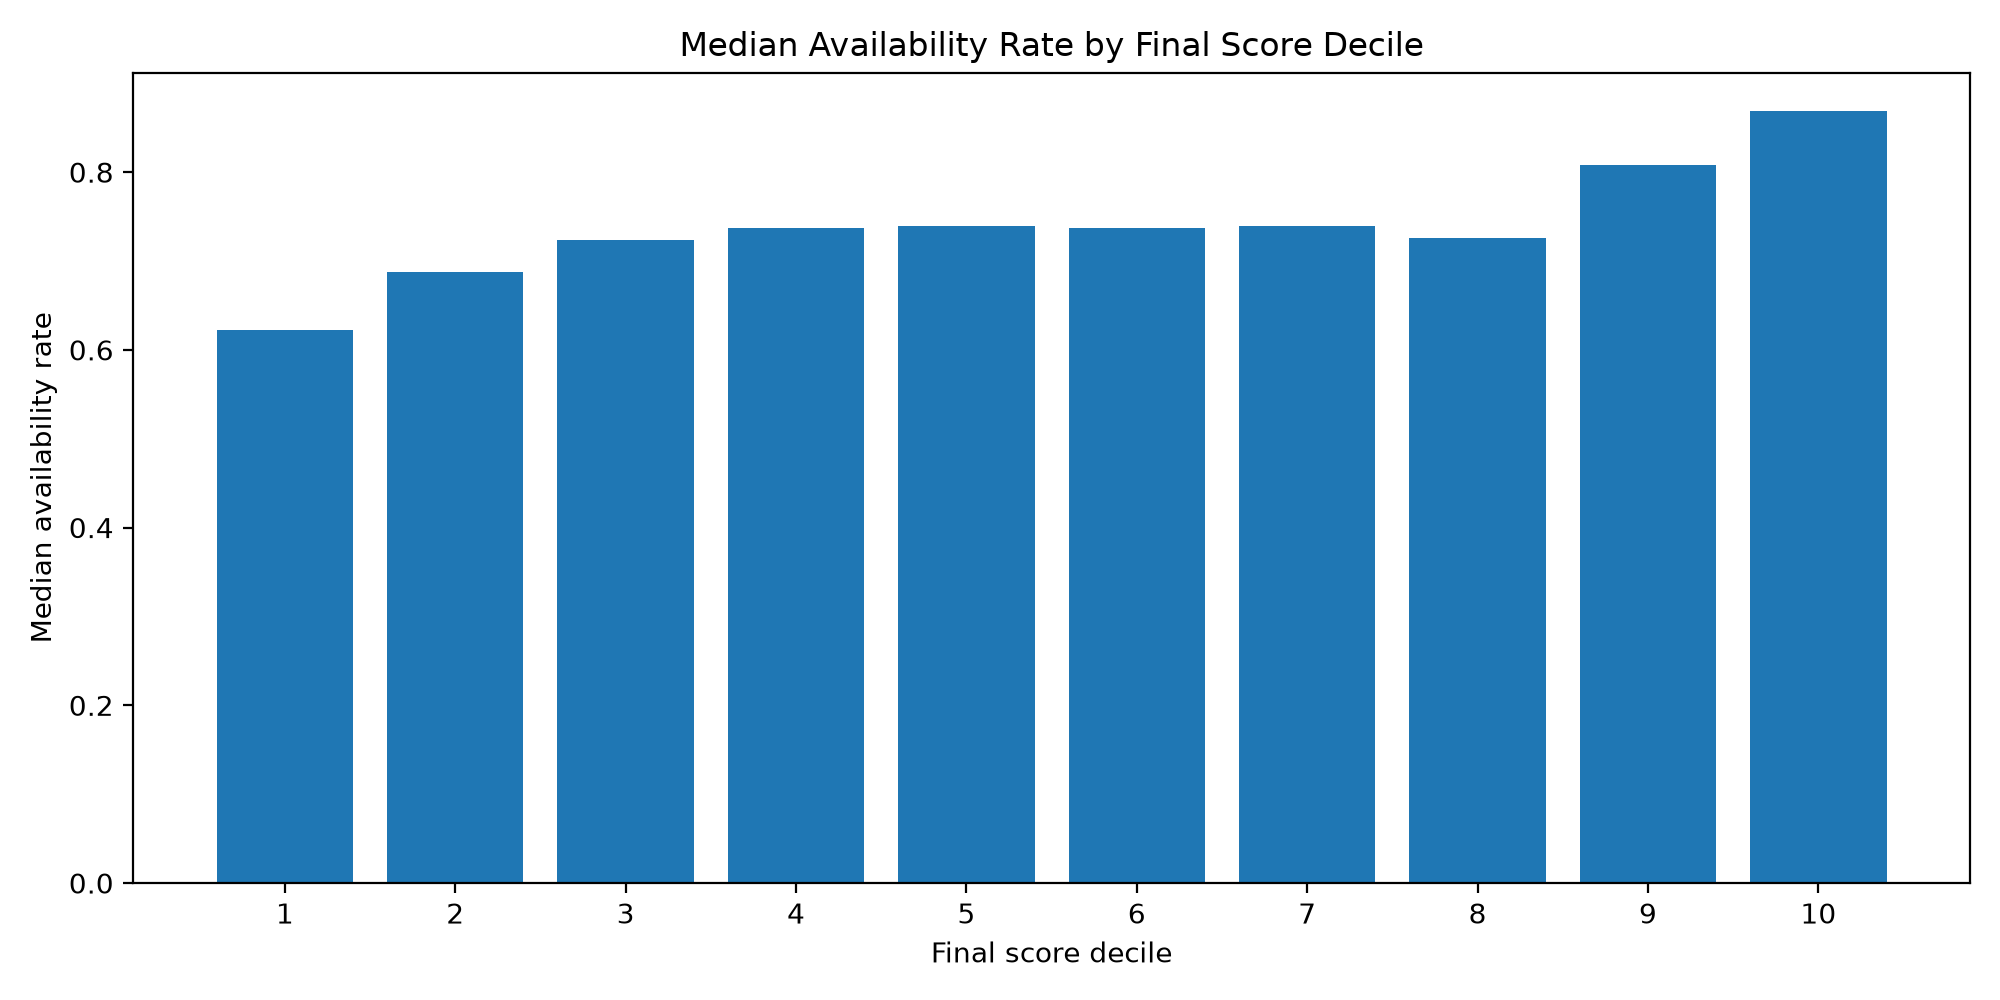
\includegraphics[width=0.76\textwidth]{figures/final/decile_vs_availability.png}
\caption{Median availability rate by final-score decile.}
\label{fig:decile_availability}
\end{figure}

For validation, I compared the selected fair-price model against simple baselines and also examined whether high-ranked listings had plausible demand-proxy patterns. The selected model improved log-RMSE by 42.48\% and dollar MAE by 37.21\% over the best baseline. The final top decile had high percent-above-expected price, high availability, and low recent reviews.

At the same time, the residual-only score had very weak Spearman correlation with availability and recent reviews. I do not view this as a failure. It means the residual model and demand-proxy layer capture different aspects of the problem. The residual says whether the listing is high relative to expected price. The availability and review variables add a separate reason to care about some of those listings more than others.

I also checked how much the top rankings overlapped when different score layers were used. The final top list was not identical to the residual-only list, especially at small cutoffs. This was expected because the final score intentionally adds cluster anomaly and demand-proxy information. The overlap becomes larger as the cutoff grows, which suggests that the broad high-risk group is more stable than the exact top few listings.

\begin{table}[H]
\centering
\caption{Overlap between top-ranked lists under different scoring views.}
\small
\begin{tabular}{rrrr}
\toprule
Top $n$ & Final vs. residual & Final vs. cluster-adjusted & Residual vs. cluster-adjusted \\
\midrule
25 & 2 & 10 & 5 \\
50 & 9 & 26 & 11 \\
100 & 25 & 66 & 24 \\
250 & 99 & 181 & 97 \\
\bottomrule
\end{tabular}
\end{table}

I did not treat the final labels as statistically proven overpricing labels, because there is no ground-truth label in the data. The stronger claim is more modest: the held-out price model performs much better than simple baselines, and the final ranking gives a reasonable screening list based on price residuals, peer comparison, feature-space anomaly, availability, and review activity.

\begin{figure}[H]
\centering
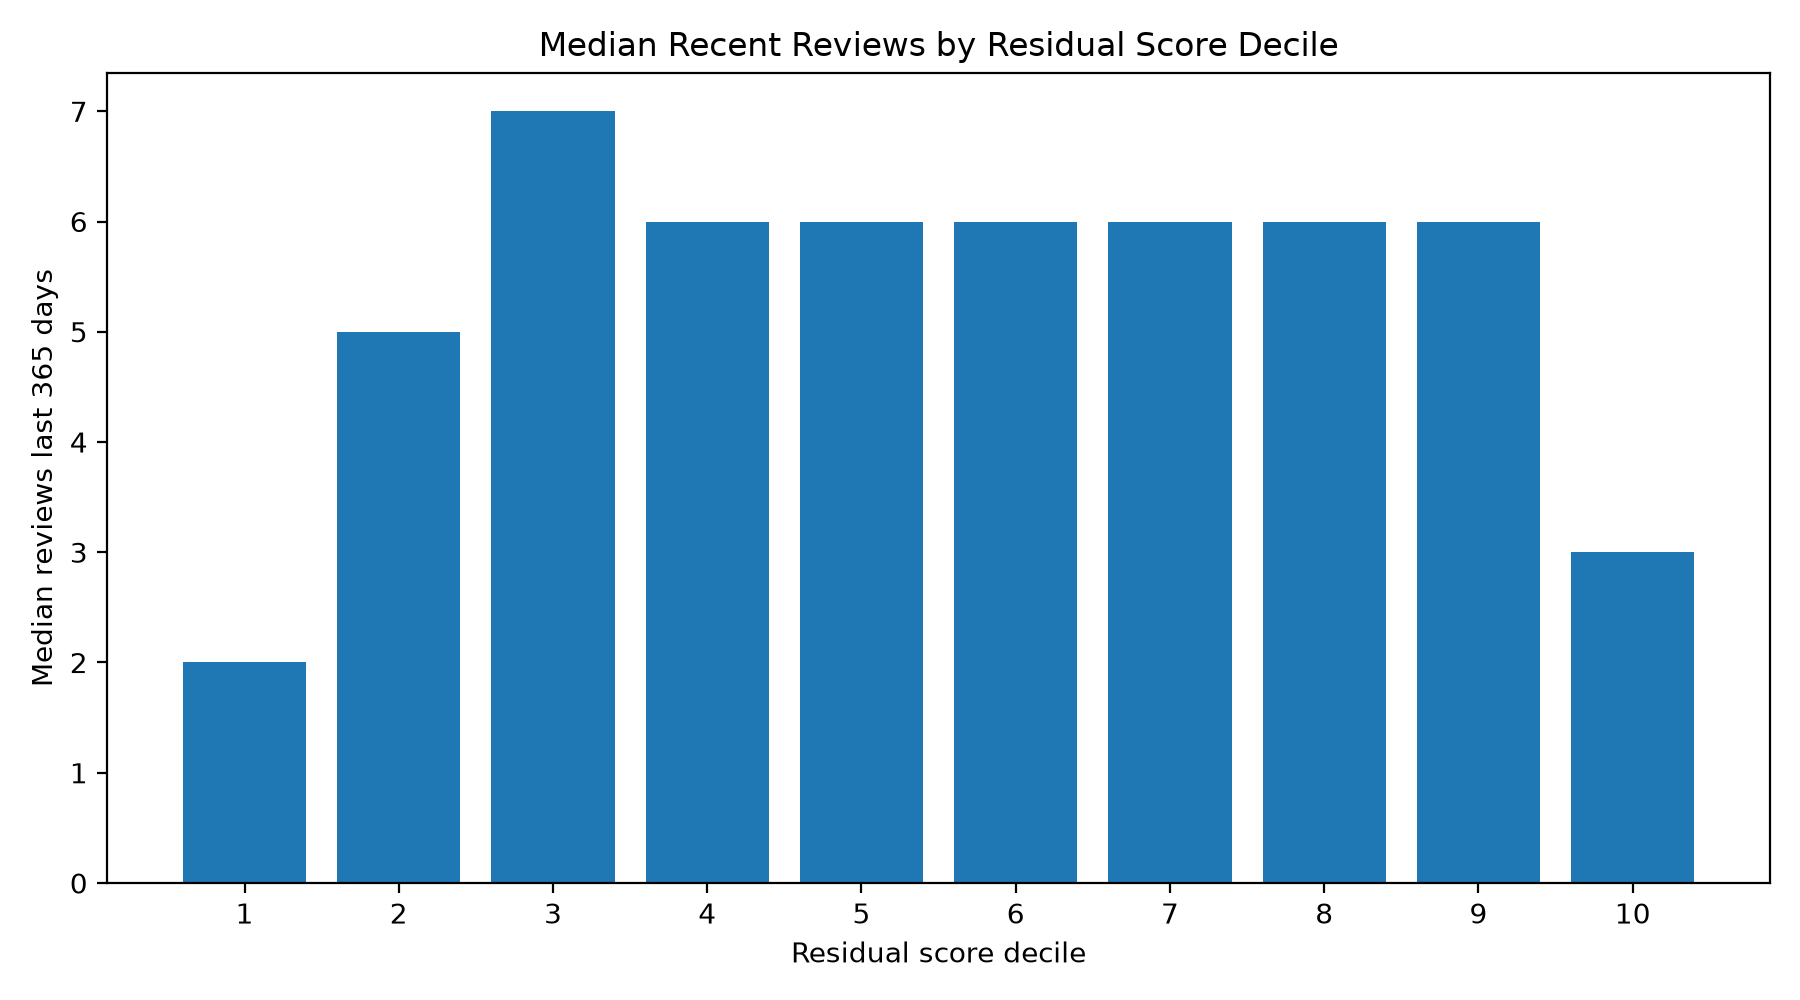
\includegraphics[width=0.76\textwidth]{figures/final/validation_residual_decile_reviews.png}
\caption{Median recent reviews by residual-score decile. Residuals alone are not the same as demand weakness, which is why the final score treats demand proxies as a separate layer.}
\label{fig:residual_reviews}
\end{figure}

\begin{landscape}
\thispagestyle{empty}
\begin{table}[H]
\centering
\scriptsize
\caption{Top final overpricing candidates. Listing names are included only to make the examples easier to interpret.}
\resizebox{\linewidth}{!}{%
\begin{tabular}{rllrrrrrr}
\toprule
Listing ID & Name & Room type & Actual price & Predicted price & Price gap & \% above expected & Final score & Label \\
\midrule
1686647652004411820 & Cozy home in NW Austin & Entire home/apt & \$2464.58 & \$294.84 & \$2169.74 & 735.90\% & 98.18 & Strong \\
1270139225068079799 & Spacious Clean Safe 1 Bedroom 9mins from COTA & Entire home/apt & \$799.00 & \$151.65 & \$647.35 & 426.89\% & 97.71 & Strong \\
1324915536546818363 & Charming Home & Private room & \$916.00 & \$482.04 & \$433.96 & 90.03\% & 97.11 & Strong \\
1556173232192810817 & Beautiful Yacht & Entire home/apt & \$942.00 & \$277.56 & \$664.44 & 239.39\% & 97.08 & Strong \\
822081454862882995 & Casa de Sito & Entire home/apt & \$243.44 & \$115.96 & \$127.48 & 109.94\% & 96.71 & Strong \\
842066613080484785 & Luxury condo on Rainey Street & Entire home/apt & \$65.08 & \$27.42 & \$37.66 & 137.34\% & 96.68 & Strong \\
1404349270335192843 & WFH-Friendly Gem, Pool Access & Entire home/apt & \$279.65 & \$96.57 & \$183.08 & 189.58\% & 96.23 & Strong \\
994197871776868819 & Cottage and Modern Guesthouse Central Austin & Entire home/apt & \$444.84 & \$217.22 & \$227.62 & 104.79\% & 96.18 & Strong \\
2189688 & Modern loft in the heart of E 6th & Entire home/apt & \$563.67 & \$334.54 & \$229.13 & 68.49\% & 95.89 & Strong \\
1111484069177681250 & 2 BD Condo Downtown Wynd. Austin & Private room & \$1273.33 & \$481.64 & \$791.69 & 164.37\% & 95.73 & Strong \\
\bottomrule
\end{tabular}%
}
\end{table}
\vfill
\begin{center}
\thepage
\end{center}
\end{landscape}

\section*{8. Limitations}

The main limitation is that there is no ground-truth overpricing label. A high score means that a listing looks expensive relative to the information in the dataset, not that the host made a pricing mistake. I also did not run a formal hypothesis test that proves one listing is overpriced. Instead, I used held-out prediction accuracy and rank-based checks as indirect evidence. Some flagged listings may be special cases, such as monthly rentals, event-based pricing, blocked calendars, unusually high-end properties, or listings with temporary pricing choices that are not fully explained by the available variables.

Calendar availability is also imperfect. An unavailable date may mean the unit was booked, but it may also mean the host blocked the date. Similarly, reviews are only a rough demand proxy because not every guest leaves a review. Because of this, the demand layer should be interpreted as supporting context rather than proof of weak demand.

The model also depends on what Inside Airbnb makes public. Important features such as real-time discounts, exact booking history, cleaning fees, host strategy, event dates, and guest search behavior are not fully available. The method is still useful as a ranking and screening system, but a production version would need more direct market and booking data.

\section*{9. Conclusion}

This project built a full pipeline for detecting potentially overpriced Austin Airbnb listings. The selected gradient boosting fair-price model substantially outperformed simple median baselines, giving a reasonable foundation for residual analysis. The residuals were then standardized within peer groups so that expensive listings were judged against comparable rentals rather than against the whole market. PCA, K-means, and GMM density scoring added a second unsupervised layer by identifying listings that were unusual in the feature space.

The final ranking found a small set of strong candidates and a larger watchlist. The strongest candidates had much higher actual prices than predicted prices, high availability, and little recent review activity. These results are not proof that any listing is incorrectly priced, but they form a practical and explainable screening method. The main value of the project is that it combines prediction, peer comparison, density scoring, and demand proxies into one interpretable ranking instead of stopping at a standard price-prediction model.

\begin{thebibliography}{99}
\bibitem{insideairbnb_data}
Inside Airbnb. \textit{Get the Data}. \url{https://insideairbnb.com/get-the-data/}. Accessed July 2026.

\bibitem{insideairbnb_assumptions}
Inside Airbnb. \textit{Data Assumptions}. \url{https://insideairbnb.com/data-assumptions/}. Accessed July 2026.

\bibitem{course_notes}
ISYE 6740 course lecture notes: clustering and K-means, PCA, density estimation, Gaussian mixture models and EM, and optimization.

\bibitem{friedman_boosting}
Friedman, J. H. (2001). Greedy function approximation: A gradient boosting machine. \textit{The Annals of Statistics}, 29(5), 1189--1232. \url{https://doi.org/10.1214/aos/1013203451}.

\bibitem{breiman_randomforest}
Breiman, L. (2001). Random forests. \textit{Machine Learning}, 45, 5--32. \url{https://doi.org/10.1023/A:1010933404324}.

\bibitem{esl}
Hastie, T., Tibshirani, R., and Friedman, J. (2009). \textit{The Elements of Statistical Learning: Data Mining, Inference, and Prediction}. 2nd ed. Springer. \url{https://doi.org/10.1007/978-0-387-84858-7}.

\bibitem{sklearn}
Pedregosa, F., Varoquaux, G., Gramfort, A., Michel, V., Thirion, B., Grisel, O., Blondel, M., Prettenhofer, P., Weiss, R., Dubourg, V., Vanderplas, J., Passos, A., Cournapeau, D., Brucher, M., Perrot, M., and Duchesnay, E. (2011). Scikit-learn: Machine learning in Python. \textit{Journal of Machine Learning Research}, 12(85), 2825--2830. \url{https://jmlr.org/papers/v12/pedregosa11a.html}.
\end{thebibliography}

\end{document}
